\documentclass[aspectratio=169]{beamer}

\usetheme{Madrid}

\usepackage{graphicx}
\usepackage{booktabs}
\usepackage{array}
\usepackage{xcolor}
\usepackage{tikz}

% Accent colors
\definecolor{accent}{RGB}{200,40,40}
\definecolor{greenaccent}{RGB}{40,160,80}
\definecolor{orangeaccent}{RGB}{255,150,40}
\definecolor{purpleaccent}{RGB}{150,70,210}
\definecolor{cyanaccent}{RGB}{50,190,210}

\setbeamertemplate{navigation symbols}{}
\setbeamersize{text margin left=0.6cm, text margin right=0.6cm}

\title{Maze Solver with Hazard Environment}
\subtitle{COSC 4368 --- AI Project Check-in 2}
\author{Group 15 - Marlon Melara, Ahnaf Murshid, Israel Mummay, Brittany Picazo, Osinachi Enemuoh}
\date{\today}

\begin{document}

%------------------------------------------------
\frame{\titlepage}

%------------------------------------------------
\begin{frame}{Project Goal}

\begin{itemize}
\item Reconstruct maze from provided image
\item Convert maze to a logical \textbf{64x64 grid}
\item Solve the maze without hazards
\item Load hazards into the environment
\item Demonstrate hazard behavior
\end{itemize}

\vspace{0.4cm}

Checkpoint focus: environment setup, solver, visualization, and hazard system.

\end{frame}

%------------------------------------------------
\begin{frame}{Maze Reconstruction}

\begin{columns}[T]

\column{0.38\textwidth}

\textbf{Pipeline}

\begin{itemize}
\item Extract maze from image
\item Detect wall boundaries
\item Convert into logical grid
\item Build adjacency structure
\end{itemize}

\vspace{0.25cm}

Generated files:

\begin{itemize}
\item \texttt{maze\_cells.npy}
\item \texttt{maze\_walls\_right.npy}
\item \texttt{maze\_walls\_down.npy}
\end{itemize}

\column{0.62\textwidth}
\centering
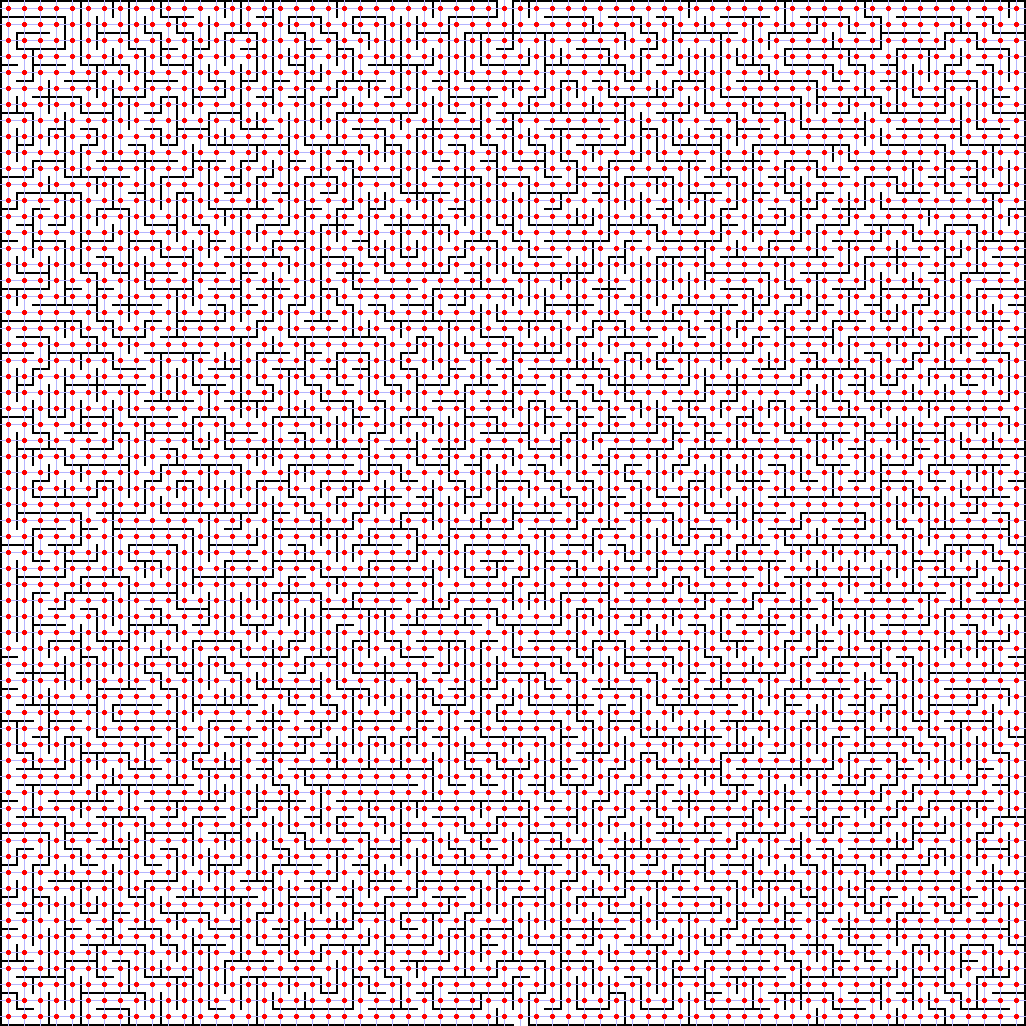
\includegraphics[width=\linewidth,height=0.66\textheight,keepaspectratio]{maze_overlay.png}

\end{columns}

\end{frame}

%------------------------------------------------
\begin{frame}{64x64 Logical Maze}
\centering
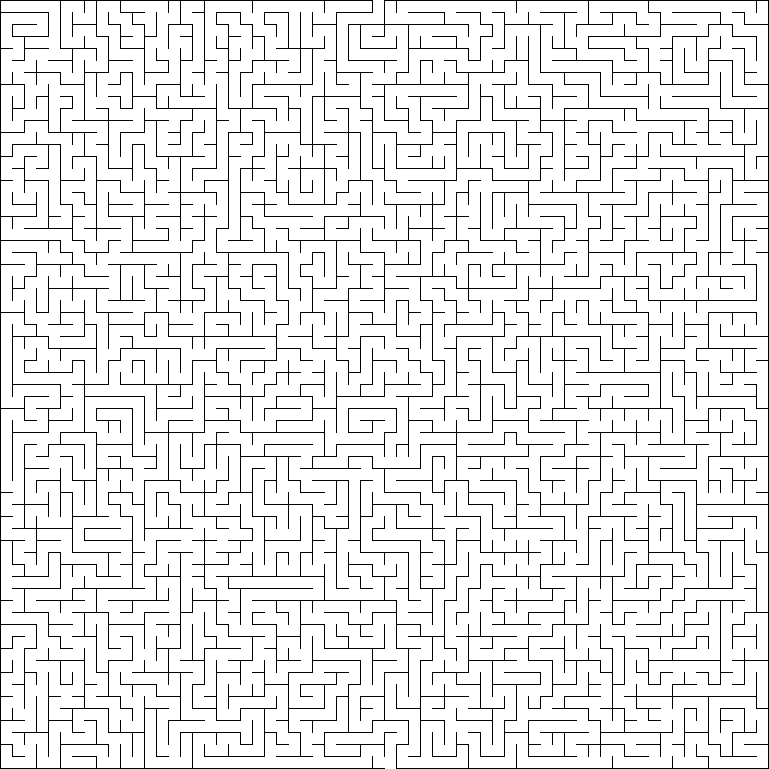
\includegraphics[width=\linewidth,height=0.72\textheight,keepaspectratio]{maze_logical_preview.png}

\vspace{0.2cm}
{\small This visualization confirms the extracted logical maze structure.}
\end{frame}

%------------------------------------------------
\begin{frame}{Naive Solver (BFS)}

\begin{columns}[T]

\column{0.38\textwidth}

Breadth First Search was used because:

\begin{itemize}
\item guarantees shortest path
\item simple and deterministic
\item ideal for grid mazes
\end{itemize}

\vspace{0.3cm}

Results:

\begin{itemize}
\item Path length: \textbf{423 cells}
\item Moves required: \textbf{422}
\item Turns (max 5 actions): \textbf{85}
\end{itemize}

\column{0.62\textwidth}
\centering
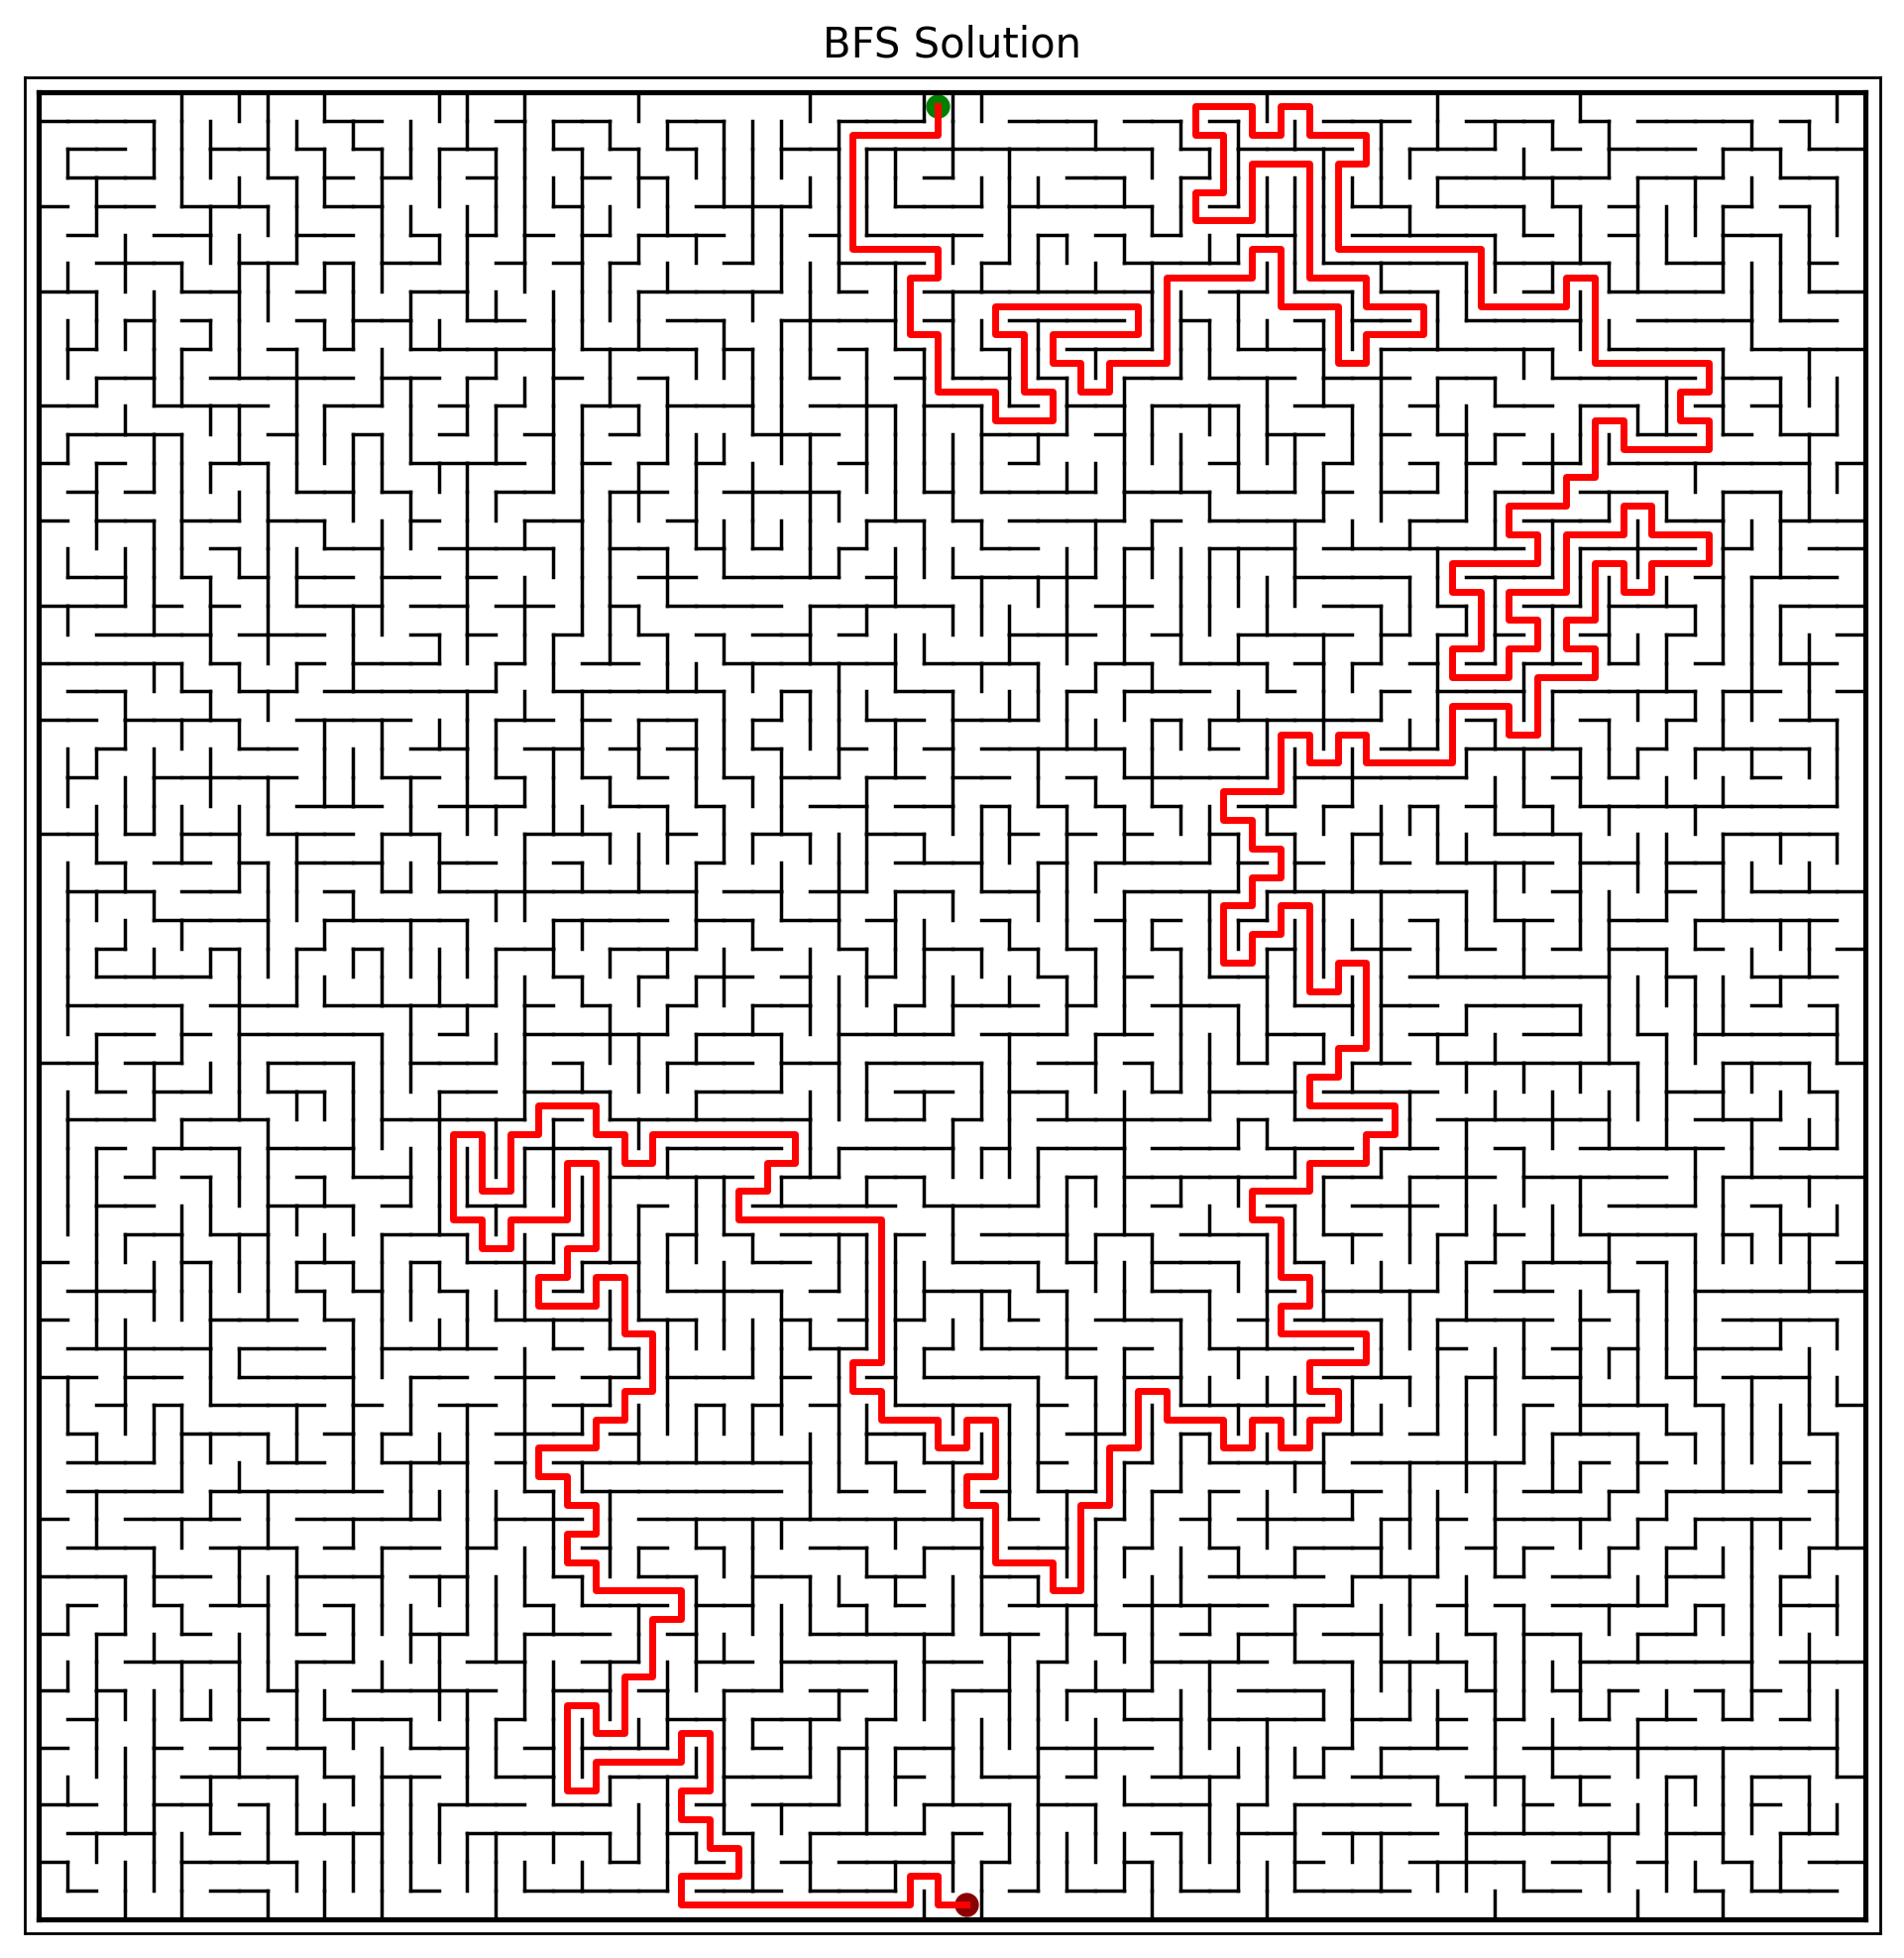
\includegraphics[width=\linewidth,height=0.66\textheight,keepaspectratio]{maze_solution.png}

\end{columns}

\end{frame}

%------------------------------------------------
\begin{frame}{Hazard System}

\begin{columns}[T]

\column{0.38\textwidth}

Three hazard types:

\textbf{Death Pits}
\begin{itemize}
\item instant death
\item respawn at start
\end{itemize}

\textbf{Teleport Pads}
\begin{itemize}
\item move agent to mapped cell
\end{itemize}

\textbf{Confusion Pads}
\begin{itemize}
\item invert controls temporarily
\end{itemize}

\vspace{0.2cm}

Hazard density:
\[
\approx 7\% \text{ of navigable cells}
\]

\column{0.62\textwidth}
\centering

\includegraphics[width=\linewidth,height=0.66\textheight,keepaspectratio]{maze_with_hazards.png}

\end{columns}

\end{frame}

%------------------------------------------------
\begin{frame}{Hazard Legend}

\begin{columns}[T]

\column{0.52\textwidth}
\centering

\includegraphics[width=\linewidth,height=0.62\textheight,keepaspectratio]{maze_with_hazards.png}

\column{0.48\textwidth}

\renewcommand{\arraystretch}{1.35}
\begin{tabular}{lll}
\toprule
Element & Marker & Meaning \\
\midrule
\tikz\fill[greenaccent] (0,0) circle (0.12); & Green circle & Start \\
\tikz\fill[accent] (0,0) circle (0.12); & Red circle & Goal \\
\textcolor{accent}{\rule{0.8cm}{1.8pt}} & Red line & BFS path \\
\tikz\fill[orangeaccent] (0,0) rectangle (0.22,0.22); & Orange square & Death pit \\
\tikz\fill[purpleaccent] (0,0) rectangle (0.22,0.22); & Purple square & Teleport pad \\
\tikz\fill[cyanaccent] (0,0) rectangle (0.22,0.22); & Cyan square & Confusion pad \\
\bottomrule
\end{tabular}

\end{columns}

\end{frame}

%------------------------------------------------
\begin{frame}{Demo Results}

\begin{itemize}
\item Maze successfully reconstructed
\item BFS solver found valid path
\item Hazard density within required range
\item Death pit demo triggered correctly
\item Teleport demo triggered correctly
\item Confusion demo triggered correctly
\end{itemize}

\vspace{0.5cm}

The system now behaves as a grid-world AI environment.

\end{frame}

%------------------------------------------------
\begin{frame}{Next Steps}

Future work:

\begin{itemize}
\item Implement intelligent navigation agents
\item Hazard-aware path planning
\item Reinforcement learning exploration
\end{itemize}

\vspace{0.6cm}

\centering
\Large Questions?

\end{frame}

\end{document}